\documentclass{exam}

\usepackage{amsmath,amssymb,amsfonts,amsthm,dsfont}
\usepackage{lib/extra}
\usepackage{graphicx}
\usepackage{tikz}
\usepackage{enumitem}
\usepackage{pgfplots}
\pgfplotsset{compat = 1.18}

\title{ST 421 HW 6}
\author{Brandyn Tucknott}
\date{22 November 2024}

\begin{document}
\maketitle

\begin{questions}
    \textbf{5.3 }
Of nine executives in a business firm, four are married, three have never married, and two are divorced. Three of the executives are selected for the promotion. Let $Y_1$ denote the number of married executives and $Y_2$ denote the number of never married executives among the three selected for promotion. Assuming that the three are randomly selected from the nine available, find the joint probability function of $Y_1, Y_2$.

\sol
Here, we let $m$ be the number of married people chosen, $n$ the number of never married people chosen. Then we count the ways we can choose married people, never married people, and the rest, and multiply their counts together. Dividing by the number of ways to choose 3 from 9 people will give us the joint probability function.
$$P\paren{Y_1 = m, Y_2 = n} = \frac{\binom{4}{m}\binom{3}{s}\binom{2}{3 - m - n}}{\binom{9}{3}}$$

\newpage
\textbf{5.5 }
The joint density of $Y_1$, the proportion of the capacity of the tank that is stocked at the beginning of the week, and $Y_2$, the proportion of the capacity sold during the week is given by
$$f(y_1, y_2) =
\begin{cases}
    3y_1, & 0 \leq y_2 \leq y_1 \leq 1 \\
    0, & \text{elsewhere} \\
\end{cases}$$

\begin{parts}
    \part
    Find $F\paren{\frac{1}{2}, \frac{1}{3}} = P\paren{Y_1 \leq \frac{1}{2}, Y_2 \leq \frac{1}{3}}$
    \sol
    $$F\paren{\frac{1}{2}, \frac{1}{3}} = \int_0^{\frac{1}{3}}\int_{y_2}^{\frac{1}{2}} 3y_1dy_1dy_2 = \int_0^{\frac{1}{3}}\frac{3}{2}\paren{\frac{1}{4} - y_2^2}dy_2 = \int_0^\frac{1}{3} \frac{3}{8}dy_2 - \int_0^\frac{1}{3} \frac{3}{2}y_2^2dy_2 = \frac{1}{8} - \frac{1}{54} = \frac{23}{216}$$
    
    
    \part
    Find $P\paren{Y_2 \leq \frac{Y_1}{2}}$, the probability that the amount sold is less than half the amount purchased.
    \sol
    $$P(Y_2 \leq \frac{Y_1}{2}) = \int_0^\frac{1}{2} \int_{2y_2}^1 3y_1dy_1dy_2 = \int_0^\frac{1}{2} \frac{3}{2}(1 - 4y_2^2)dy_2 = \frac{3}{2}\paren{y_2 - \frac{4}{3}y_2^3}\Bigg|_0^\frac{1}{2} = \frac{1}{2}$$
\end{parts}

\newpage
\textbf{5.6 }
If a radioactive particle is randomly located in a square of unit length, a reasonable model for the joint density function $Y_1, Y_2$ is

$$f(y_1, y_2) =
\begin{cases}
    1, & 0 \leq y_1, y_2 \leq 1 \\
    0, & \text{elsewhere} \\
\end{cases}$$

\begin{parts}
    \part
    What is $P(Y_1 - Y_2 > 0.5)$?
    \sol
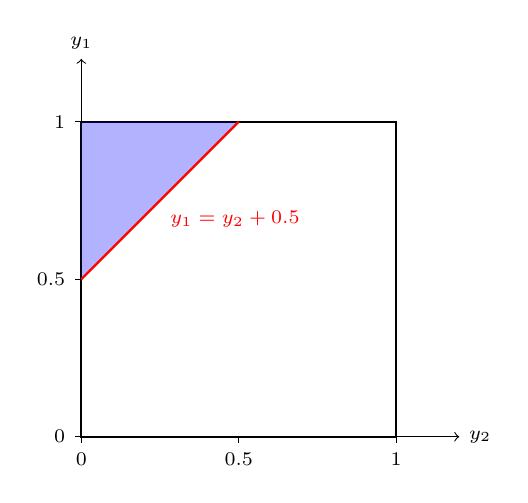
\begin{tikzpicture}[scale=4, every node/.style={font=\scriptsize}]

% Draw the unit square
\draw[very thin, gray] (0,0) grid (1,1);
\draw[thick] (0,0) rectangle (1,1);

% Label axes
\draw[->] (0,0) -- (1.2,0) node[right] {$y_2$};
\draw[->] (0,0) -- (0,1.2) node[above] {$y_1$};

% Shade the area above the line
\fill[blue, opacity=0.3] (0.5,1) -- (0,1) -- (0,0.5);


% Slope 1 line
\draw[red, thick] (0,0.5) -- (0.5,1) node[pos=0.5, below right] {$y_1 = y_2 + 0.5$};

% Tick marks
\foreach \x in {0, 0.5, 1} {
    \draw (\x,0) -- (\x,-0.02) node[below] {\x};
    \draw (0,\x) -- (-0.02,\x) node[left] {\x};
}

\end{tikzpicture}
\newline
$$P(Y_1 - Y_2 > 0.5) = \frac{\text{area of triangle region}}{\text{area of unit square}} = \frac{0.5\cdot (0.5\cdot 0.5)}{1\cdot 1} = \frac{1}{8}$$

    
    \part
    What is $P(Y_1Y_2 < 0.5)$?
    \sol
\begin{tikzpicture}
    \begin{axis}[
        xlabel={$y_1$},
        ylabel={$y_2$},
        xmin=0, xmax=1,
        ymin=0, ymax=1,
        axis lines=middle,
        samples=100,
        domain=0.001:1, % Avoid division by zero
        restrict y to domain=0:1, % Restrict y_2 within bounds
        legend pos=north east,
        xtick={0, 0.5, 1}, % Custom ticks on x-axis
        ytick={0, 0.5, 1}, % Custom ticks on y-axis
        grid=both
    ]
        % Plot the function
        \addplot[blue, thick] {1 / (2 * x)};
        \legend{$y_2 = \frac{1}{2y_1}$}
        
        % Dotted line for y_1 = 1
        \addplot[dotted, thick] coordinates {(1, 0) (1, 1)};
        
        % Dotted line for y_2 = 1
        \addplot[dotted, thick] coordinates {(0, 1) (1, 1)};
    \end{axis}
\end{tikzpicture}
    $$P(Y_1Y_2 < 0.5) = P\paren{Y_1 < 0.5\cdot \frac{1}{Y_2}} = \frac{3}{4} + \int_\frac{1}{2}^1\int_\frac{1}{2}^{y_2} 0.5y_1dy_1dy_2 = \frac{3}{4} + 0.5\int_\frac{1}{2}^1 \ln y_2 + \ln 2dy_2 =$$

    $$= \frac{3}{4} + \frac{\ln 2}{4} + 0.5\cdot\paren{y_2\ln y_2 - y_2}\Bigg|_\frac{1}{2}^1 = \frac{3}{4} + \frac{\ln 2}{4} + 0.5\paren{(0 - 1) - \paren{\frac{-\ln 2}{2} - \frac{1}{2}}} =$$
    
    $$\frac{3}{4} + \frac{\ln 2}{4} + \frac{1}{2}\paren{\frac{\ln 2}{4} - \frac{1}{2}} = \frac{3}{4} + \frac{\ln 2}{4} + \frac{\ln 2}{4} - \frac{1}{4} = \frac{1}{2} + \frac{\ln 2}{2} \approx 0.8466$$
    
\end{parts}

\newpage
\textbf{5.9 }
Let $Y_1. Y_2$ have the joint probability density function given by
$$f(y_1, y_2) =
\begin{cases}
    k(1 - y_2), & 0 \leq y_1 \leq y_2 \leq 1 \\
    0, \text{elsewhere} \\
\end{cases}$$

\begin{parts}
    \part
    What is the value of $k$ that makes this a probability density function?
    \sol
    $$\int_0^1 \int_0^{y_2} k(1 - y_2)dy_1dy_2 = \int_0^1 ky_2(1 - y_2)dy_2 = \frac{k}{6}$$

    But recall this integral should be 1, so we set it equal to one and solve for $k$, giving us $k = 6$.


    \part
    Find $P\paren{Y_1 \leq \frac{3}{4}, Y_2 \geq \frac{1}{2}}$
    \sol
    $$P\paren{Y_1 \leq \frac{3}{4}, Y_2 \geq \frac{1}{2}} = \int_\frac{3}{4}^1 \int_0^\frac{3}{4} 6(1 - y_2) dy_1dy_2+ \int_\frac{1}{2}^\frac{3}{4} \int_0^{y_2} 6(1 - y_2) dy_1dy_2 = 0.4844$$
    
    
\end{parts}




\newpage
\textbf{5.23 }
Consider the joint density function of $Y_1$, the proportion of the capacity of the tank that is stocked at the beginning of the week, and $Y_2$, the proportion of the capacity sold during the week given by
$$f(y_1, y_2) =
\begin{cases}
    3y_1, & 0 \leq y_2 \leq y_1 \leq 1 \\
    0, & \text{elsewhere} \\
\end{cases}$$

\begin{parts}
    \part
    Find the marginal density function for $Y_2$.
    \sol
    The marginal density function of $Y_2$ is integrating the joint density function for all variables except $Y_2$. In this case, it is just $Y_1$.
    $$f_{Y_2}(y_2) = \int_{y_2}^1 3y_1 dy_1 = \frac{3y_1^2}{2}\Bigg|_{y_2}^1 = \frac{3}{2} - \frac{3y_2^2}{2}$$

    \part
    For what values of $y_2$ is the conditional density$f(y_1 | y_2)$ defined?
    \sol
    $$f(y_1 | y_2) = \frac{f(y_1, y_2)}{f_{Y_2}(y_2)} = \frac{3y_1}{\frac{3}{2}(1 - y_2^2)} = \frac{2y_1}{1 - y_2^2}$$
    So $f(y_1 | y_2)$ is defined as long as $y_2 \neq 1$.

    \part
    What is the probability that more than half a tank is sold given three-fourths of the tank is stocked?
    \sol
    $$f\paren{Y_1 \geq \frac{1}{2} | Y_2 = \frac{3}{4}} = \int_\frac{1}{2}^\frac{3}{4} \frac{2y_1}{1 - \paren{\frac{3}{4}}^2} dy_1 = \frac{2\cdot 16}{7} \int_\frac{1}{2}^\frac{3}{4} y_1 dy_1 = \frac{32}{7}\paren{\frac{y_1^2}{2}}\Bigg|_\frac{1}{2}^\frac{3}{4} =$$

    $$= \frac{32}{7}\paren{\frac{9}{32} - \frac{1}{8}} = \frac{35}{256} \approx 0.7143$$

    
\end{parts}



\newpage
\textbf{5.25 }
Let $Y_1, Y_2$ have the joint density function
$$f(y_1, y_2) =
\begin{cases}
    e^{-(y_1 + y_2)}, & y_1, y_2 > 0 \\
    0, & \text{elsewhere} \\
\end{cases}$$

\begin{parts}
    \part
    Find the marginal density functions for $Y_1$ and $Y_2$. Identify these densities as one of those studied in chapter 4.
    \sol
    $$f_{Y_1}(y_1) = \int_0^\infty e^{-y_1 - y_2} dy_2 = \paren{-e^{-y_1 - y_2}}\Bigg|_0^\infty = e^{-y_1}, \text{and by symmetry}$$

    $$f_{Y_2}(y_2) = e^{-y_2}$$

    \part
    What is $P(1 < Y_1 < 2.5)$ and $P(1 < Y_2 < 2.5)$?
    \sol
    Since the joint density function is symmetrical, we note that $P(1 < Y_1 < 2.5) = P(1 < Y_2 < 2.5)$. Arbitrarily, we compute the probability $Y_1$ is within this range.
    $$P(1 < Y_1 < 2.5) = \int_0^{2.5} f_{Y_1}(y_1)dy_1 - \int_0^1 f_{Y_1}(y_1)dy_1 = \int_0^{2.5} e^{-y_1} dy_1 - \int_0^1 e^{-y_1} dy_1 =$$

    $$= \paren{-e^{-y_1}}\Bigg|_0^{2.5} - \paren{-e^{-y_1}}\Bigg|_0^1 = \paren{-e^{-2.5} - 1} - \paren{-e^{-1} - 1} = -e^{-2.5} + e^{-1} \approx 0.2858$$

    \part
    For what values of $y_2$ is the conditional density $f(y_1 | y_2)$ defined?
    \sol
    $$f(y_1 | y_2) = \frac{\text{joint}}{\text{marginal of }y_2} = \frac{e^{-y_1 - y_2}}{e^{-y_2}} = e^{-y_1}$$

    From this, we know that for all values of $y_2$, the conditional density $f(y_1 | y_2)$ is defined.

    \part
    For any $y_2 > 0$, what is the conditional density function of $Y_1$ given $Y_2 = y_2$?
    \sol
    As shown in Part (c), $f(y_1 | y_2) = e^{-y_1}$.

    \part
    For any $y_1 > 0$, what is the conditional density function of $Y_2$ given $Y_1 = y_1$?
    \sol
    By symmetry, $f(y_2 | y_1) = e^{-y_2}$

    \part
    For any $y_2 > 0$, how does the conditional density function $f(y_1 | y_2)$ that you obtained in Part (d) compare to the marginal density function found in Part (a)?
    \sol
    We found that the conditional function of $Y_1$ given $Y_2$ is equivalent to the marginal function of $Y_1$.

    \part
    What does your answer in Part (f) imply about marginal and conditional probabilities that $Y_1$ falls in any interval?
    \sol
    $f(y_1 | y_2) = f_{Y_1}(y_1)$ tells us that $Y_1, Y_2$ are independent. As a result, the probability that $Y_1$ falls in any interval is independent of $Y_2$.
    
\end{parts}




\newpage
\textbf{5.43 }
Let $Y_1, Y_2$ have joint density function $f(y_1, y_2)$ and marginal densities $f_1(y_1)$ and $f_2(y_2)$ respectively. Show that $Y_1$ and $Y_2$ are independent if and only if $f(y_1 | y_2) = f_1(y_1)$ for all $y_1, y_2 s.t. f_2(y_2) > 0$.
\begin{proof}
Recall that two random variables are independent if and only if $f(x, y) = f_X(x)\cdot f_Y(y)$. \\

First, we show that if $Y_1, Y_2$ are independent, then $f(y_1 | y_2) = f_2(y_2)$. Independence gives us
$$f(x, y) = f_1(y_1)\cdot f_2(y_2) \longrightarrow \frac{f(x, y)}{f_2(y_2)} = f_1(y_1)\longrightarrow$$

$$f(y_1 | y_2) = f_1(y_1) \text{ if } f_2(y_2) > 0$$

Next, we show that if $f(y_1 | y_2) = f_1(y_1)$ and $f_2(y_2) > 0$, then $Y_1,Y_2$ are independent.
$$f(y_1 | y_2) = f_1(y_1) \text{ and } f_2(y_2) > 0 \longrightarrow$$

$$\frac{f(x, y)}{f_2(y_2)} = f_1(y_1) \longrightarrow$$

$$f(x, y) = f_1(y_1)\cdot f_2(y_2)$$

This is the definition of independence, so we are done. We conclude that $Y_1, Y_2$ are independent if and only if $f(y_1 | y_2) = f_1(y_1)$ with $f_2(y_2) > 0$.
\end{proof}

\newpage
\textbf{5.64 }
Let $Y_1, Y_2$ be independent random variables that are both uniformly distributed along the interval $(0, 1)$. Find $P(Y_1 < 2Y_2 | Y_1 < 3Y_2)$
\sol
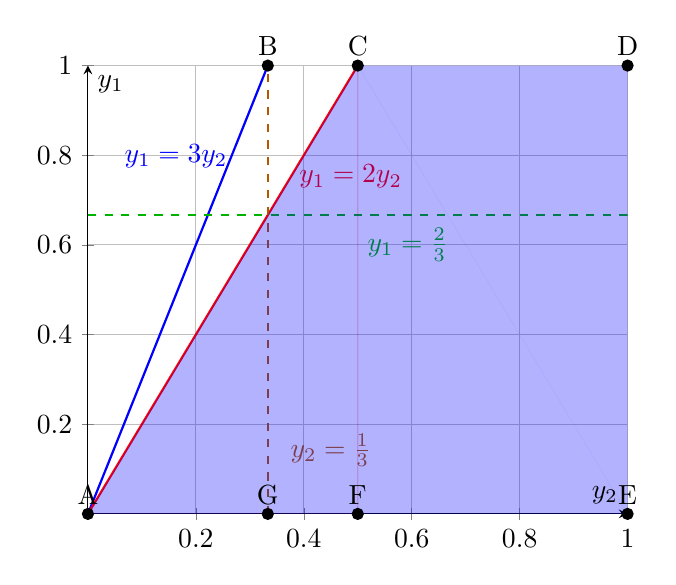
\begin{tikzpicture}
    \begin{axis}[
        axis lines=middle,
        xlabel={$y_2$},
        ylabel={$y_1$},
        xmin=0, xmax=1,
        ymin=0, ymax=1,
        xtick={0,0.2,...,1},
        ytick={0,0.2,...,1},
        grid=both,
        legend style={at={(0.02,0.98)}, anchor=north west, draw=none}
    ]
        % Line y1 = 3y2
        \addplot[domain=0:0.33, thick, blue] {3*x};
        \node[anchor=south west, blue] at (axis cs:0.05,0.75) {$y_1 = 3y_2$};
        
        % Line y1 = 2y2
        \addplot[domain=0:0.5, thick, red] {2*x};
        \node[anchor=north east, red] at (axis cs:0.6,0.8) {$y_1 = 2y_2$};
        
        % Line y1 = 2/3
        \addplot[domain=0:1, thick, dashed, green!70!black] {2/3};
        \node[anchor=west, green!70!black] at (axis cs:0.5,0.6) {$y_1 = \frac{2}{3}$};
        
        % Line y2 = 1/3
        \addplot[domain=0:1, thick, dashed, orange!70!black] coordinates {(1/3, 0) (1/3, 1)};
        \node[anchor=north, orange!70!black] at (axis cs:0.45,0.2) {$y_2 = \frac{1}{3}$};

        % Shaded region below y1 = 2y2
        \addplot[domain=0:0.5, red, opacity=0.2, samples=100] {2*x} \closedcycle;

        \fill[blue, opacity=0.3] (0, 0) -- (0.5, 1) -- (1, 0);
        \fill[blue, opacity=0.3] (0.5, 1) -- (1, 0) -- (1, 1);

        % Add specific points
        \addplot[
            only marks,
            mark=*,
            mark options={black},
            nodes near coords,
            point meta=explicit symbolic % For custom labels
        ] coordinates {
            (0, 0)[A] % Point A
            (0.3333, 1)[B] % Point B
            (0.5, 1)[C] % Point C
            (1, 1)[D] % Point D
            (1, 0)[E] % Point E
            (0.5, 0)[F] % Point F
            (0.3333, 0)[G] % Point G
        };
    \end{axis}
\end{tikzpicture}

\newline
In order to solve for this, we use Baye's formula.
$$P(Y_1 < 2Y_2 | Y_1 < 3Y_2) = \frac{P(Y_1 < 3Y_2 | Y_1 < 2Y_2)P(Y_1 < 2Y_2)}{P(Y_1 < 3Y_2)} =$$

Since the random variables are uniformly distributed, we can simply find the ratios of the areas as our answer.


$$\frac{\text{Area( ACF )} + \text{Area( CDEF )}}{\text{Area( ABG )} + \text{Area( BDEG )}} = \frac{1\cdot \paren{\frac{1}{2}\cdot \frac{1}{2}\cdot 1} + \frac{1}{2}\cdot 1}{\paren{\frac{1}{2}\cdot \frac{1}{3}\cdot 1} + \frac{2}{3}\cdot 1} = \frac{\frac{3}{4}}{\frac{5}{6}} = \frac{9}{10}$$
\end{questions}

\end{document}